\section{State of the art in silicon-level operating ESD investigation}

Section \ref{sec:state-art-esd-testing} introduced major \gls{esd} standards used in laboratories to test and qualify electronic products.
Sometimes, discharges propagate inside electronic equipments, reach the integrated circuits and cause them to malfunction.
It is essential to detect early functionnal weaknesses against \gls{esd}.
This section reviews the litterature on the current state of the art on operating \gls{esd} analysis.
Study cases, observation methods and modeling approaches are presented.
Ultimately, the goal is to debug efficiently the behavior of integrated circuits in operation when they are exposed to \gls{esd}.

\subsection{Study cases}

% Case 1 - NXP bandgap + substrate coupling
The case of an alternator's regulator \gls{ic} is presented in \cite{softfailEMCIC}.
where a product is investigated and designed for high immunity against electromagnetic disturbances.
The failure signature is a loss of the regulated voltage.
It was proven that the disturbance was coupling through the substrate on a current mirror inside the bandgap.
During the disturbance, bandgap voltage was shifting from its nominal value, causing a full system restart.
A design fix was proposed by filtering at the appropriate spot inside the design to avoid the amplification of the disturbance.
%TODO: Investigation method ?

% Case 2 - CESAME IC - paper Vrignon + Ben dhia
Another failure case is presented in \cite{LacrampeTransientImmunity}.
Very-fast \gls{tlp} is injected on an 0.18 \textmu{}m CMOS technology (1.8 V supply voltage) chip.
The chip contains 6 instances on the same logic core, differing by their power-rails architecture.
The injection on the power rail is performed by a 1 nF capacitor, similarly to the \gls{dpi} standard \cite{iec62132-4}.
% What is the failure signature
An output signal of the logic core is monitored.
The susceptibility criteria is the amplitude crossing a 20\% threshold from the established logic level.
Above this threshold, the core is supposed to no longer work reliably.
It is proven that modelling the output buffer of the core logic can reproduce with less than 20\% error the waveform on the output.
It is less accurate than a full-netlist simulation, but faster to simulate.
VHDL-AMS and SPICE modelling are performed in this analysis.

% Case 3 - failures on an SDRAM
%TODO: Read reference articles in this article
In \cite{SDRAMCase}, soft-failures are studied on a SDRAM memory in operation.
The injection setup consists in a modified \gls{tem} cell with a reduced septum height for increased field strenghts.
The SDRAM chip is mounted on a board.
Data is written and read on the memory by \gls{fpga}.
Differences between incoming and outgoing data signifies a functional failure of the memory.
Only the memory is exposed to the disturbance, the rest of the board's devices are located outside of the \gls{tem} cell, on the other side of the board.
The main defect of this method is to only provide a global failure level.
It does not allow to identify which particular net or pin is the most sensitive to disturbances.

In \cite{softFailSubsystem}, electrostatic discharges cause errors on two different camera communication buses.
Events of different severities are observed, depending on the discharge parameters.
It is attempted to determine whether the sensor or the application processor is causing the error.
The magnetic emission map is recorded with a near-field magnetic scanner to try to observe local variations in the emission spectrum because of the degradation of functionnality.
It was envisionned that soft-failure can induce significant variations in the emission spectrum of a disturbed component, and thus those variations could help localize them.
In this particular case, the root cause of failures could not be determined.

An LCD display is studied in \cite{softFailLCD}.
The device is tested with an IEC 61000-4-2 \cite{iec61000-4-2} generator, and non-destrutive problems are observed due to the discharge.
Electromagnetic disturbances cause stripes to appear on the display, optical parameters changes and blacklighting malfunctions.
System-level testing waveforms were found too complex for identifying the root cause.
A near-field injection is performed to identify which trace of the LCD's flex connector claims the lowest immunity.
The lack of resolution of the near-field probe caused multiple traces to be disturbed at once, preventing this second approach to work.
Finally, the individual track stressing was repeated with a capacitively-coupled \gls{tlp} on each individual metal track.
However, results were once more unconclusive and no metal trace could categorically be identified as more sensitive than the others.
The conclusion for this paper is that silicon level soft-error models are required for standard investigation.

An investigation method is presented in \cite{softFailMobile} to search for discharge propagation paths responsible for soft-failures on a mobile phone.
The IEC 61000-4-2 standard is chosen as testing waveform.
Metallic parts are assumed to be the main propagation paths.
To confirm this hypothesis, electromagnetic 3D simulations of the entire phone are ran.
After the failure location was determined, RC-networks are used as countermeasures to protect physical inputs and outputs, like buttons, LCD inputs and connectors.

\subsection{Observation methods for failure detection and localisation}

\subsubsection{Emmission Microscopy (EMMI)}

%TODO: References
% Concept
\gls{emmi} is an observation technique where a camera registers photon emission above semiconductor devices.
A device is placed in the field of view of the camera.
The entire system is placed inside an enclosure to block out all ambient light.
The device is powered up.
Semiconductor junctions and defects emit photons when electrically excitated.
By letting the camera shutter open for a long time, between a few hundred milliseconds to tens of seconds, photons generated by this process are detected by the image sensor.
As photons accumulate, some sections of the image become brighter than others.
Defects can be isolated from normal junctions by comparing recordings performed on tested devices with a reference device.
The architecture of an \gls{emmi} system is provided in Fig. \ref{fig:emmi}.

\begin{figure}[!h]
  \centering
  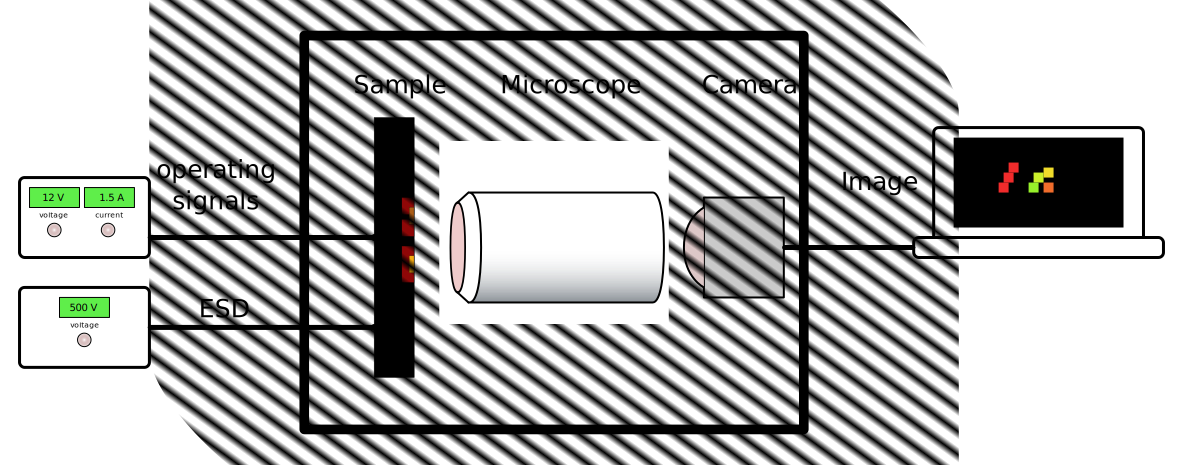
\includegraphics[width=0.3\textwidth]{src/1/figures/architecture_emmi.pdf}
  \caption{Architecture of an emmi testbench}
  \label{fig:emmi}
\end{figure}

% In ESD field
%TODO: Find more uses
\gls{emmi} is presented in \cite{softfailEMMI} as a successful analysis method for debugging and locating a functional failure on an integrated circuit exposed to \gls{esd}.
Fig. \ref{fig:emmi-examples} shows two different images recorded with an \gls{emmi} bench.
The image on the left is... and the one on the right is....

\begin{figure}[!h]
  \centering
  \includegraphics[width=0.3\textwidth]{src/1/figures/examples_emmi.pdf}
  \caption{Images recorded from an EMMI measurement}
  \label{fig:emmi-examples}
\end{figure}

\subsubsection{Near-field scanner}

Electromagnetic near-field scanner is a system able to measure a spatial map of the electrical and magnetic field.
It usually consists in performing a sweep closely above a device with an electric or magnetic probe to record the emitted field in near conditions.
Similarly to \gls{emmi}, the generated map is very useful to locate failures and malfunctions in a device or system.
A comprehensive analysis of the near-field measurement technique is done in \cite{nfsFirstStudy}.
More recent work detail the principles, data processing and hardware requirements for building such kind of equipment \cite{planarNFSAntenna, NFSMeasurements, NFScanner}.
The architecture of a near-field scanner is given in Fig. \ref{fig:near-field-scanner}.

\begin{figure}[!h]
  \centering
  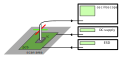
\includegraphics[width=0.3\textwidth]{src/1/figures/architecture_near_field_scanner.pdf}
  \caption{Architecture of a near-field scanning testbench}
  \label{fig:near-field-scanner}
\end{figure}

\subsection{Particular test methods}

In the litterature, some particular test methods have been presented, comprising for instance of new test generators or modified injections methods.
This section gathers a few of them that are relevant for powered-on \gls{esd} testing.

% Reduced TEM cell
A more compact \gls{tem} cell is proposed in \cite{SDRAMCase}.
The reduced dimensions lead to higher electrical fields, to reach levels normally produced by an \gls{esd} gun.
The discharge waveform, injected inside the cell, is generated by a filtered \gls{tlp} and is similar in shape to IEC 61000-4-2 \cite{iec61000-4-2}.

% Near-field scan as injection tool
Near-field scanner is usually a measurement tool, but it can also serve as a localized stress injection system.
Instead of sensing voltage or current in the near-field probe, a pulse is injected in it.
In \cite{NearFieldInjectionFabrice}, a near-field scanner is combined with a very fast \gls{tlp} to test local immunity of a device.
This methods yields an immunity map, that highlights sensitive areas of a board.
The paper demonstrates that it is possible to map quantitatively and with good resolution the \gls{esd} susceptibility of a board with this method.
In a similar approach, \gls{esd} sensitive metal tracks and \gls{ic} pins are identified in \cite{NearFieldInjectionBis} with a near-field scanner in the same injection configuration.

%TODO: Search more particular methods

\subsection{Modeling methods of soft-failures for integrated circuits}

A lot of work has been presented in the litterature regarding electromagnetic modeling and simulation.

% TODO: read article again
Mixed mode ESD simulations \cite{mixedModeESDSims}.

% TODO: read article again
SEED methodology ? in \cite{usb2ESDProtection}.
Interactions between external devices leading to soft-failures and how to fix them ?

% TODO: What is the goal ?
3D EM simulation \cite{LacrampeTransientImmunity} at silicon level, with the integrated circuit layout.
Deduce capacitive couplings between Vdd and Vss rails
Model by equivalent impedance
Method is complex and long to simulate ? but was proven to work effectively to model parasitic couplings.
Alternative to parasitic device extraction directly from layout.
IBIS package data was employed to model the package by an RLC equivalent

%
Modelling of a TLP stress generator in \cite{LacrampeTransientImmunity} using a lookup table I(V) component, in series with a 50\textOmega{} resistor.

% TODO: Interest of the EM simulation ?
Electromagnetic fullwave simulations are conducted in \cite{softFailMobile}.
System-level components are simulated, such as PCB, metallic casing and battery back.

% Modelling of IC input pin from a TLP characterization
Proven in \cite{usb2ESDProtection} that a TLP characterization I(V) curve of an IC pin can be used to model it for a (signal ?) kind of input.

% IBIS is not enough for modelling an IC pin for ESD simulations
Input Output Buffer Information Specification (IBIS) \cite{ibis-spec} is a method for digital circuits providing the I/V characteristic of an IC without disclosing any circuit or process information.
IBIS provides a behavioral modeling technique for digital circuits for performing signal integrity simulation.
The idea is to characterize and distribute information about the package, buffers and protection diodes (not ESD protections), not the IC core.
It is demonstrated in \cite{ibisImprovementFabrice} that for EMC and ESD simulations the model is not sufficient.
It is not defined for fast impulses and high injection.
